%++++++++++++++++++++++++++++++++++++++++
% Don't modify this section unless you know what you're doing!
\documentclass[letterpaper,11pt]{article}

%%%%%%%%%%% ADICIONEI
\usepackage{booktabs}
\usepackage{multirow}
\usepackage{siunitx}
\usepackage{subfigure}
\usepackage{subcaption}


%%%%%%%%%%%

\usepackage{natbib}
\bibliographystyle{unsrtnat}
\usepackage{tabularx} % extra features for tabular environment
\usepackage{amsmath}  % improve math presentation
\usepackage{graphicx} % takes care of graphic including machinery
\usepackage[margin=1in,letterpaper]{geometry} % decreases margins
%\usepackage{cite} % takes care of citations
\usepackage[final]{hyperref} % adds hyper links inside the generated pdf file
\hypersetup{
	colorlinks=true,       % false: boxed links; true: colored links
	linkcolor=blue,        % color of internal links
	citecolor=blue,        % color of links to bibliography
	filecolor=magenta,     % color of file links
	urlcolor=blue         
}
%+++++++++++++++++++++++++++++++++++++++
\begin{document}

\title{Data Science \& Machine Learning - Deliverable 02 - Slot 04. \\\textbf{Mini Projeto - Wallmart}}
\author{Saul de Azevêdo Souza, RID: 33259\\
 Guilherme Marinho De Araujo, RID: 38445}
\date{\today}
\maketitle

\begin{abstract}
Neste \textbf{'Deliverable - slot 04'} utilizamos um Dataset sobre vendas semanais de lojas estadunidenses. O objetivo era indicar o melhor investimento para a Wallmart. Aqui, foi de fundamental importância utilizar ferramentas para análise estatística de dados por meio do Python. Além disso, procuramos seguir todo o processo de gerenciamente de projetos envolvido em ciência de dados, como o CRISP-DM. Para obter os resultados, seguimos entendendo todas as etapas do processo. Após o entendimento, partimos para a análise dos dados. Esta etapa englobou diferentes ferramentas para análise estatística de dados e a tomada de decisão foi feita com auxilio de uma métrica de negócio (mediana das vendas semanais). Por fim, sugerimos a loja 4 com base em um conjunto de filtros e pela métrica de negócio.

\end{abstract}

\section{Introdução}%Projeto - Deliverable 01 - Slot 03}
Somos uma empresa especializada em pesquisa quantitativa e fornecemos suporte em análise estatística de dados e tomada de decisão para pessoas físicas e outras empresas. É importante destacar que nossa tomada de decisão é baseada em informações obtidas a partir de dados (muitas vezes fornecidos pelos clientes). Destacamos que os procedimentos estatísticos utilizados buscam ao máximo possível reduzir ou controlar a probabilidade  de se cometer qualquer tipo de erro relacionado a pesquisa.

\subsection{A Questão de Negócio}

Recentemente fomos contratados pela Wallmart para fazer um levantamento do faturamento das lojas nos USA e apontar qual loja seria melhor para expandir seu tamanho. Por ainda esta dando os primeiros passos e adequando as políticas da empresa para os processos tecnológicos, precisa de suporte para reduzir os risco na exposição de novos investimentos. Como parte de sua estratégia, a Wallmart pretende investir em lojas nos Estados Unidos e precisa de informações suficientes para embasar sua tomada de decisão.

Quanto aos objetivos, a Roof Imóveis espera que possamos fornecer uma consultoria estratégica de modo a:
\begin{itemize}
    \item (i) Fazer um levantamento dos faturamento de lojas nos Estados Unidos;
    \item (ii) Determinar qual dessas lojas ela deve investir.
\end{itemize}

A escoha da loja deve ser feita de modo a reduzir o risco do investimento. Para atender os objetivos traçados, planejamos fazer uma análise descritiva dos dados a fim de estudar o comportamento das vendas semanais dessas lojas. Essa estrategia permitirá ter uma noção das variáveis que impactam negativamente nas vendas, causando um maior risco ao negócio.

\subsection{O Entendimento do Negócio}

Walmart, Inc., é uma multinacional estadunidense de lojas de departamento. A companhia foi fundada por Sam Walton em 1962, incorporada em 31 de outubro de 1969 e feita capital aberto na New York Stock Exchange, em 1972. 

No ano de 2021, obteve um um lucro de \$ 13.51 Bilhões.
Sendo uma das principais lojas de varejo do mundo. Os dados contemplam as vendas semanais de 45 lojas espalhadas pelos Estados Unidos. O Walmart realiza vários eventos promocionais de descontos ao longo do ano. Essas remarcações precedem feriados importantes, os quatro maiores de todos, que são o Super Bowl, o Dia do Trabalho, o Dia de Ação de Graças e o Natal. As semanas que incluem esses feriados têm um peso maior.

Os dados fornecidos são relevantes para o problema e correspondem as características de vendas semanais das lojas e outras referentes a sua localização, por exemplo, a taxa de desemprego da região. Essas informações são uteis para determinar quais lojas apresentam um maior risco de investimento com base nas vendas semanais e das caractetísticas atreladas ao imóvel.

\subsection{A Coleta de Dados}

Como citado anterioremente, o Dataset utilizado apresenta as vendas semanais de 05/02/10 até 01/11/12 em 45 lojas varejistas da rede Wallmart e também algumas métricas econômicas e meteriológicas por semana. A descrição destas características estão abaixo. A priori não foi necessário calcular nenhuma informação por fora. Ou seja, os dados foram suficientes para a tomada de decisão.

Para estes dados, esperamos que as variáveis tenham um maior correlacionamento com as vendas semanais. Também podemos utilizar alguma variável para tentar segmentar/filtrar melhor os dados. O Dataset não possui observações não informadas, registradas como Null ou NA. Por sua vez, os outliers podem ser identificados a partir dos gráficos de boxplot.

\subsection{A Limpeza de Dados}

Neste projeto, os dados podem ser baixados em um único arquivo compactado, acessado a partir do seguinte endereço eletrônico 
\begin{itemize}
    \item  \textbf{https://www.kaggle.com/yasserh/walmart-dataset}.
\end{itemize}

O arquivo em específico, nomeado por \textbf{wallmart.csv}, contém resgistros das vendas semanais separados por vírgulas (formato CSV). Essa será nossa fonte principal de dados para as análises subsequentes. Neste projeto, os procedimentos computacionais foram desenvolvidos utilizando a linguagem de programação \textbf{Python}.

\subsection{Descrição dos dados}

A Tabela~\ref{table1} apresenta uma breve descrição das variáveis utilizadas neste estudo. Ela apresenta 8 variáveis referentes as vendas, métricas econômicas e meterológicas por semana. Além disso, é destacado o formato em que os dados foram salvos no arquivo. É possível destacar uma variável em formato \textbf{object}. Logo, deve ser convertida em formato numérico para análise posterior.  As variáveis econômicas podem ser relacionadas com as vendas para determinarmos o grau de correlação linear entre elas. Por sua vez, é possível verificar se as vendas aumentam significativamente nos feriados.

\begin{table}[!htb]

\begin{center}
\caption{Descrição e tipo das variáveis fornecidas no DataSet.}

\label{table1} 
\begin{tabular}{clc} %change to cc for 2 columns
\hline
\multicolumn{1}{c}{Variáveis } & \multicolumn{1}{c}{Definição} & Tipo da variável \\
\hline
Store &  Id/número da loja&  int64  \\
Date & semana de venda &  \textbf{object}  \\
Weekly\_Sales& venda naquela semana &  float64  \\
Holiday\_Flag& indica se é ou não feriado naquela data (1 se for feriado; 0 caso contrário) & int64  \\
Temperature& temperatura do dia em $^{\circ} F$ &  float64  \\
Fuel\_Price&   preço do combustível na região da loja  & float64\\
CPI&   índice de preços ao consumidor  & float64\\
Unemployment& taza de desemprego &  float64  \\

\hline
\end{tabular}
\end{center}
\end{table}

A Figura~\ref{fig1} apresenta algumas estatísticas descritivas, como: mínimo (min), primeiro quartil (25\%), mediana (50\%), média (mean), desvio padrão (std), terceiro quartil (75\%) e máximo (max) das variáveis utilizadas. Essas estatísticas são baseadas em 6435 observações. Algumas conclusões podem ser feitas através de sua análise. Por exemplo, as vendas semanais apresentam uma grande variabilidade dado o alto valor de desvio padrão (564366.6). Para melhorar a qualidade dos dados, é possível pensar em agrupar as informações por lojas. Para isso, precisaremos utilizar alguma medida de agrupamento como média/mediana. Entender a variabilidade das vendas acaba se tornando um fator importante uma vez que queremos lojas que tenham uma certa constância em vendas. Ou seja, pouca variabilidade

\begin{figure}[!htb] 
\caption{\label{fig1}Estatística descritiva das variáveis utilizadas.
        }
        \centering 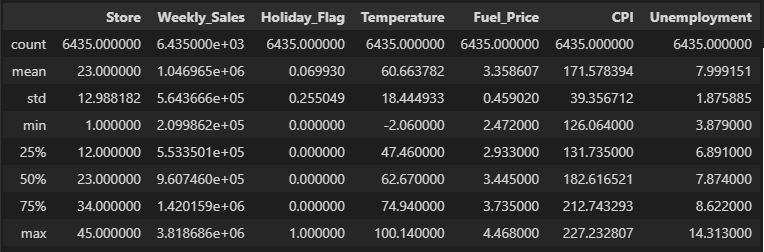
\includegraphics[width=1\columnwidth]{descritiva.png}
        
\end{figure}

Outro ponto importante é verificar os possíveis relacionamentos, caso existam, entre as vendas e as demais variáveis quantitativas. Isso permitirá verificar quais variáveis impactam negativamente as vendas semanais.

A Tabela~\ref{table33} a seguir apresenta o coeficiente de correlacão de Pearson. Podemos verificar que as correlação com vendas não são altas, chegando a ser fracas. Vale destacar que as variáveis CPI, Unemployment e Temperature estão correlacionadas negativamente com Weekly\_Sales. Ou seja, quando seus valores aumentam as vendas semanais tendem a diminuir. A variável Fuel\_Price, por sua vez, apresenta uma correlação linear bem próxima a zero. Logo, é interessante construir um diagrama de dispersão para saber se existe outração função diferente de $y = x$ que consiga explicar a relação entre elas.

\begin{table}[!htb]
\begin{center}
\caption{Coeficiente de correlação linear para a variável vendas semanais.}
\label{table33} 
\begin{tabular}{cccccccccccc} 
\hline
Variáveis & Correlação ($r$ de Pearson) \\
\hline
Temperature	&-0.063810 \\
Fuel_Price& 0.009464 \\
CPI& -0.072634\\
Unemployment	& -0.106176 \\

\hline
\end{tabular}
\end{center}
\end{table}

\subsection{Visualização dos dados}

Uma maneira prática e rápida de visualizar o comportamento dos dados é através de figuras. A Figura~\ref{fig:uu} apresenta os gráficos de dispersão que cruzam o escore de uma variável com o escore de outra variável. Aqui, podemos perceber que:
\begin{itemize}
    \item a variável CPI segmenta de forma natural as vendas semanais e podemos perceber uma maior nuvem de pontos para valores de CPI menores do que 145. Ou seja, uma região com maior quantidade de vendas;
    \item a variável fuel\_price também pode ser utilizada para segmentar as vendas. Isto por que para preços de gasolina menores do que 3.75 existem uma maior concetração de vendas com possibilidades de vendas atipicas. 
    \item Para valores de temperatura entre 20 e 60 $^{\circ}F$ existe um maior volume de vendas, incluindo vendas atípicas.
    \item Por fim, para valores de taxa de desemprego menores do que 10 existe uma maior concentração de observações, favorecendo também o surgimento de vendas atípicas.
\end{itemize}


\begin{figure}[!htb]
  \centering
  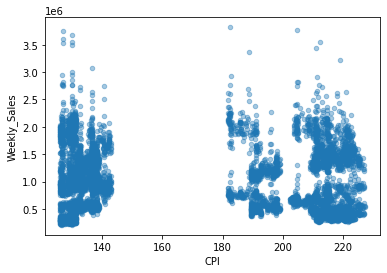
\includegraphics[width=.49\linewidth]{cpi.png}
  \label{fig:sfig1}
  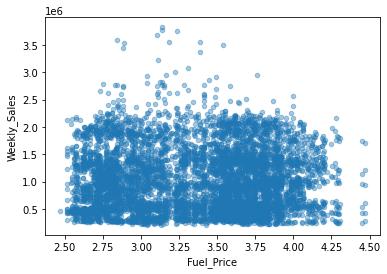
\includegraphics[width=.49\linewidth]{fuel_price.png}
  \label{fig:sfig2}
  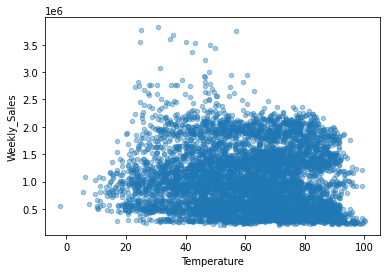
\includegraphics[width=.49\linewidth]{temperature.png}
  \label{fig:sfig2}
  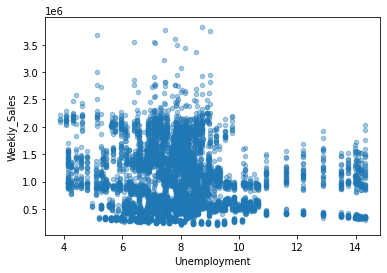
\includegraphics[width=.49\linewidth]{unemployment.png}
  \label{fig:sfig2}
  \caption{Gráfico de dispersão dos escores das variáveis quantitativas contra os escores das vendas semanais.}
\label{fig:uu}
\end{figure}

Os pontos destacados na análise acima podem ser utilizados como filtros para faciliar a seleção do melhor investimento. Entendemos que lojas situadas em regiões pouco favorecidas, quanto as variáveis analisadas, apresentam um menor número de vendas e não costumam ter vendas atípicas. Logo, os filtros ajudam a controlar esse risco, filtrando lojas que estão em regiões com menores impostos, temperaturas agradáveis aos consumidores, pequena taxa de desemprego e um preço de combustível atrativo ao consumidor.

Para avaliar o comportamento das vendas semanais por loja podemos construir um boxplot. A ideia é visualizar as lojas que apresentam pouca variabilidade (constância em vendas ao longo das semanas) e uma mediana de vendas alta (mostrando que ela tende a ter  valores elevados de vendas). A Figura~\ref{fig22} mostra que a loja 4 apresenta uma mediana elevada e uma variabilidade menor do que boa parte das lojas. Por sua vez, as lojas 33 e 44 apresentam pequenos valores de vendas semanais e acabam sendo excluidas pelo filtro definido acima.

\begin{figure}[!htb] 
        \centering 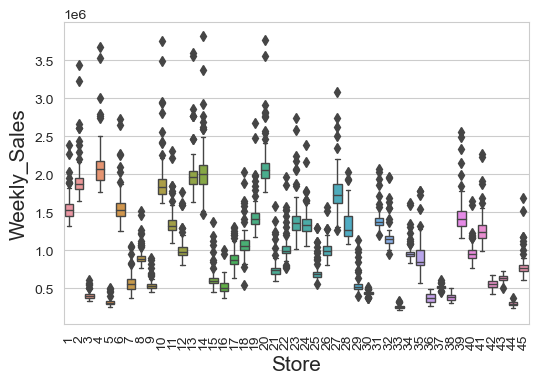
\includegraphics[width=0.5\columnwidth]{boxplot.png}
        \caption{\label{fig22}Boxplot das vendas semanais por loja.
        }
\end{figure}

\subsection{Métricas do negócio}

Para definirmos qual a melhor loja, precisamos controlar os riscos. Entendemos como risco aquela loja que apresenta pequeno volumes de vendas decorrente das condições econômicas e meterológicas fornecidas pelo Dataset. Então, os filtros podem ser utilizados para reduzir esses riscos, excluindo do Dataset aquelas lojas que estão fora de certas especificações. Essas especificações são definidas a partir da análise gráfica na Figura~\ref{fig:sfig2}. Nesta análise procuramos uma região de valores das covariáveis que apresentam grandes valores de vendas (entenda como concentração de pontos) com presença de valores atípicos (considerados bons, pois aumentam as vendas).

A Figura~\ref{fig223} apresenta o boxplot das vendas semanais após aplicar os filtros. Podemos perceber uma redução no número de lojas. Aqui, escolheremos aquela loja que apresenta a maior mediana de vendas mensais (métrica do negócio) em conjunto com uma pequena variabilidade (constância em vendas).

\begin{figure}[!htb] 
        \centering 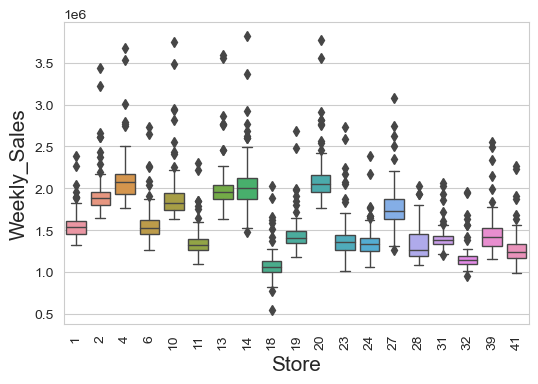
\includegraphics[width=0.5\columnwidth]{boxplotfinal.png}
        \caption{\label{fig223}Boxplot das vendas semanais por loja após aplicar a filtragem nos dados (removendo lojas com certo risco).
        }
\end{figure}

A Figura~\ref{fig224} apresentamos a loja 4 como o melhor investimento. Para isso ordenamos as lojas em ordem decrescente de mediana. Ou seja, a loja 4 passou por todos os filtros de risco e foi selecionada por apresentar a maior mediana de vendas, além de ter uma das menores variabilidades.

\begin{figure}[!htb] 
        \centering 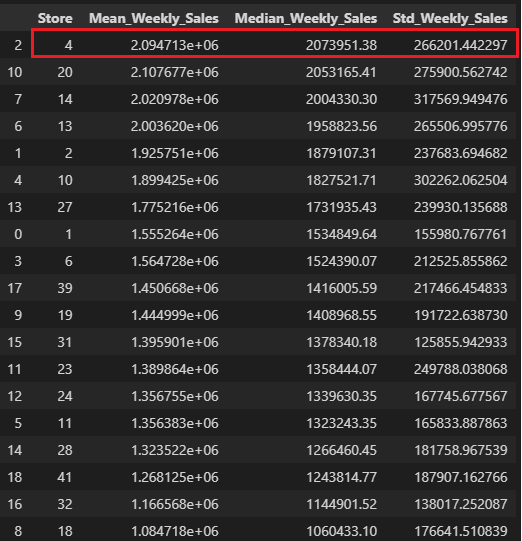
\includegraphics[width=0.5\columnwidth]{metrica.png}
        \caption{\label{fig224}Resultado do ordenamento das lojas segundo a maior mediana de vendas semanais.
        }
\end{figure}

\section{Tomada de decisão}

A tomada de decisão foi feita seguindo um critério quantitativo. Ou seja, selecionamos o melhor investimento com base na mediana das vendas semanais, excluindo do Dataset as lojas mais arriscada. Aqui, entendemos como arriscado aquelas lojas que tem um pequeno faturamento, influenciado ate certo ponto pelas covariáveis abordadas no estudo.

\end{document}
